\begin{figure}[t]
\centering
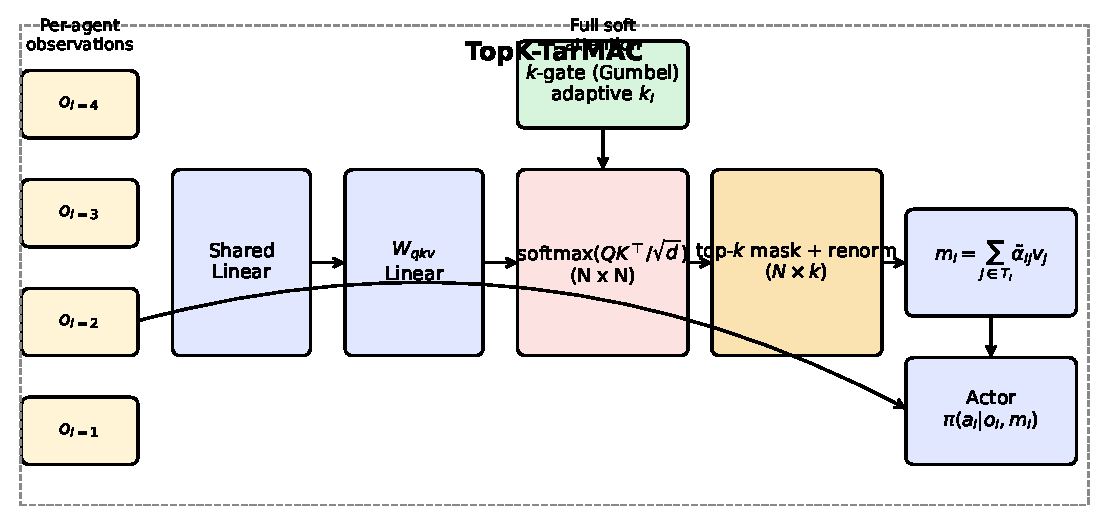
\includegraphics[width=0.92\linewidth]{figures/fig1_schematic.pdf}
\caption{TopK-TarMAC architecture. Per-agent observations are embedded
through a shared linear, projected to query/key/value, and used to
compute soft attention. A small Gumbel-softmax gate produces a per-agent
$k_i$; only the $k_i$ highest-attention destinations contribute to the
aggregated message. The reduce-to-baseline switch (zero out $m_i$)
recovers MAPPO exactly.}
\label{fig:schematic}
\end{figure}

\paragraph{Setup.} We consider a cooperative Dec-POMDP with $N$ agents,
local observations $o_i$, shared state $s$, joint action $a = (a_1, \ldots,
a_N)$, and team reward $r(s, a)$. Following MAPPO \citep{yu2022mappo}, we
train a parameter-shared actor $\pi_\theta(a_i \mid o_i, m_i)$ that also
conditions on a message vector $m_i$ produced by an inter-agent attention
module, and a centralised critic $V_\phi(s)$ trained against the
team-reward GAE return.

\paragraph{Dense attention baseline (TarMAC-style).} Each agent embeds its
observation $e_i = \mathrm{GELU}(W_e o_i)$, and emits a query/key/value
triple $(q_i, k_i, v_i) = W_{qkv} e_i$. Scaled dot-product attention is
computed pairwise with the self-attention diagonal masked:
\begin{equation}
  \alpha_{ij} = \frac{\exp(\langle q_i, k_j\rangle / \sqrt{d})\,[i\neq j]}
               {\sum_{j'\neq i} \exp(\langle q_i, k_{j'}\rangle/\sqrt{d})}.
\end{equation}
The dense channel aggregates over all peers:
$m_i^{\text{dense}} = W_o\,\mathrm{GELU}\!\left(\sum_{j\neq i} \alpha_{ij} v_j\right)$.
Cost: $\mathcal{O}(N^2 d)$ score + $\mathcal{O}(N^2 d)$ aggregation per step.

\paragraph{TopK-TarMAC.} We compute the same soft attention scores $\alpha$
but aggregate only the $k$ entries of highest score per row, then
renormalise:
\begin{align}
  \mathcal{T}_i &= \mathrm{top}_k\!\left(\{\alpha_{ij}\}_{j\neq i}\right), \\
  \tilde{\alpha}_{ij} &= \frac{\alpha_{ij}\,[j \in \mathcal{T}_i]}
                       {\sum_{j'\in\mathcal{T}_i}\alpha_{ij'}}, \\
  m_i^{\text{topk}} &= W_o\,\mathrm{GELU}\!\left(\sum_{j\in\mathcal{T}_i}
                                                   \tilde\alpha_{ij} v_j\right).
\end{align}
Aggregation cost falls to $\mathcal{O}(N k d)$ per step.

\paragraph{Adaptive $k$.} Rather than fixing $k$ globally, we let each agent
choose its own $k_i \in \{1, \ldots, N{-}1\}$ from a small gate
$g_i = W_g e_i \in \mathbb{R}^{N-1}$, sampled with Gumbel-softmax with
hard one-hot output:
\begin{equation}
  p_i = \mathrm{Gumbel\text{-}Softmax}(g_i,\, \tau, \, \text{hard}=\text{True}).
\end{equation}
At training time, gradients flow through the soft Gumbel via the
straight-through trick; at evaluation time, $k_i = \arg\max p_i$ is taken
hard. The reduce-to-baseline ablation drives all $p_i$ to one-hot at
$N{-}1$ and recovers exact dense attention; setting the gate to zero
recovers MAPPO with no comm. We verify this property as a unit test of
the implementation.

\paragraph{Objective and training.} The actor + critic are trained with
MAPPO's clipped surrogate
\citep{yu2022mappo, schulman2017ppo}; no auxiliary loss is added on the
attention or gate output, so any preference for sparsity must emerge from
the task signal alone. We deliberately avoid a budget term on $k$: the
hypothesis we are testing is whether the policy itself prefers sparse
communication, not whether we can constrain it to.
